% ---- pg-053 （书页 41） ----
看得很清楚:若 $|c|>1$,则 $\bm{x}$ 延长;若 $0<|c|<1$,则 $\bm{x}$ 缩短[回顾\hyperref[fig:2.2]{图 2.2}(a)].选取 $c = L_x^{-1}$,便得到长度为 1 且与 $\bm{x}$ 同方向的单位向量 $L_x^{-1}\bm{x}$.

第二个几何概念是角.考虑平面内两个向量以及它们之间的夹角 $\theta$,如\hyperref[fig:2.4]{图 2.4} 所示.由图可见,$\theta$ 可表示成这两个向量分别同第一坐标轴的夹角 $\theta_1$ 和 $\theta_2$ 之差.因为,根据定义,

\[
\cos(\theta_1) = \frac{x_1}{L_x} \qquad \cos(\theta_2) = \frac{y_1}{L_y}
\]
\[
\sin(\theta_1) = \frac{x_2}{L_x} \qquad \sin(\theta_2) = \frac{y_2}{L_y}
\]

因而

\[
\cos(\theta) = \cos(\theta_2 - \theta_1) = \cos(\theta_2)\cos(\theta_1) + \sin(\theta_2)\sin(\theta_1)
\]

两个向量 $\bm{x}' = [x_1, x_2]$ 和 $\bm{y}' = [y_1, y_2]$ 之间的夹角 $\theta$ 由下式确定:

\phantomsection\label{eq:2-3}
\begin{equation}
\cos(\theta) = \cos(\theta_2 - \theta_1) = \left(\frac{y_1}{L_y}\right)\left(\frac{x_1}{L_x}\right) + \left(\frac{y_2}{L_y}\right)\left(\frac{x_2}{L_x}\right) = \frac{x_1y_1 + x_2y_2}{L_xL_y} \tag{2-3}
\end{equation}

我们发现引进两个向量的内积是方便的.对于 $n=2$ 维情形,$\bm{x}$ 和 $\bm{y}$ 的内积为

\[
\bm{x}'\bm{y} = x_1y_1 + x_2y_2
\]

根据这个定义和\hyperref[eq:2-3]{式(2-3)},有

\[
L_x = \sqrt{\bm{x}'\bm{x}} \qquad \cos(\theta) = \frac{\bm{x}'\bm{y}}{L_xL_y} = \frac{\bm{x}'\bm{y}}{\sqrt{\bm{x}'\bm{x}}\sqrt{\bm{y}'\bm{y}}}
\]

因为 $\cos(90^\circ) = \cos(270^\circ) = 0$,且仅当 $\bm{x}'\bm{y} = 0$ 时 $\cos(\theta) = 0$,所以当 $\bm{x}'\bm{y} = 0$ 时 $\bm{x}$ 与 $\bm{y}$ 互相垂直.

对任意维数 $n$,定义 $\bm{x}$ 与 $\bm{y}$ 的内积如下:

\phantomsection\label{eq:2-4}
\begin{equation}
\bm{x}'\bm{y} = x_1y_1 + x_2y_2 + \cdots + x_ny_n \tag{2-4}
\end{equation}

内积用 $\bm{x}'\bm{y}$ 或 $\bm{y}'\bm{x}$ 表示.

利用内积,就能将 $n$ 个分量的向量的长度和夹角自然地推广为

\phantomsection\label{eq:2-5}
\begin{equation}
L_x = \bm{x} \text{ 的长度} = \sqrt{\bm{x}'\bm{x}} \tag{2-5}
\end{equation}

\phantomsection\label{eq:2-6}
\begin{equation}
\cos(\theta) = \frac{\bm{x}'\bm{y}}{L_xL_y} = \frac{\bm{x}'\bm{y}}{\sqrt{\bm{x}'\bm{x}}\sqrt{\bm{y}'\bm{y}}} \tag{2-6}
\end{equation}

还是因为仅当 $\bm{x}'\bm{y} = 0$ 时 $\cos(\theta) = 0$,所以我们说,当 $\bm{x}'\bm{y} = 0$ 时 $\bm{x}$ 与 $\bm{y}$ 互相垂直.

\mvbold{例 2.1} （计算向量的长度和它们之间的夹角）

给定向量 $\bm{x}' = [1, 3, 2]$ 和 $\bm{y}' = [-2, 1, -1]$,求 $3\bm{x}$ 和 $\bm{x} + \bm{y}$.然后确定 $\bm{x}$ 的长度,$\bm{y}$ 的长度以及 $\bm{x}$ 与 $\bm{y}$ 之间的夹角.最后检验 $3\bm{x}$ 的长度是 $\bm{x}$ 长度的 3 倍.

首先,

\[
3\bm{x} = 3\begin{bmatrix} 1 \\ 3 \\ 2 \end{bmatrix} = \begin{bmatrix} 3 \\ 9 \\ 6 \end{bmatrix}
\]

\[
\bm{x} + \bm{y} = \begin{bmatrix} 1 \\ 3 \\ 2 \end{bmatrix} + \begin{bmatrix} -2 \\ 1 \\ -1 \end{bmatrix} = \begin{bmatrix} 1 - 2 \\ 3 + 1 \\ 2 - 1 \end{bmatrix} = \begin{bmatrix} -1 \\ 4 \\ 1 \end{bmatrix}
\]

\begin{mvfigure}
\begin{tikzpicture}[scale=1.1]
\draw[->] (0,0) -- (3.6,0) node[right] {$x$};
\draw[->] (0,0) -- (0,2.6) node[above] {$y$};
\draw[->] (0,0) -- (2.6,1.5) node[right] {$\bm{y}$};
\draw[->] (0,0) -- (3.0,1.0) node[above right] {$\bm{x}$};
\draw (0.9,0) arc (0:22:0.9);
\draw (1.2,0) arc (0:30:1.2);
\node at (1.35,0.16) {$\theta_2$};
\node at (1.75,0.30) {$\theta$};
\node at (0.55,0.35) {$\theta_1$};
\node[left] at (0,2.0) {$y_2$};
\node[below] at (2.0,0) {$x_2$};
\node[below] at (0.95,0) {$y_1$};
\node[below] at (2.85,0) {$x_1$};
\draw[dashed] (0,1.5) -- (2.0,1.5);
\draw[dashed] (2.0,0) -- (2.0,1.5);
\draw[dashed] (0,1.0) -- (1.0,1.0);
\draw[dashed] (1.0,0) -- (1.0,1.0);
\node at (1.9,1.85) {$\cos(\theta) = \dfrac{x_1y_1 + x_2y_2}{L_xL_y}$};
\end{tikzpicture}
\phantomsection\label{fig:2.4}\mvcap{图 2.4\quad $\bm{x}' = [x_1, x_2]$ 与 $\bm{y}' = [y_1, y_2]$ 之间的夹角 $\theta$}
\end{mvfigure}
